\documentclass[svgnames,hyperref, french, xcolor=dvipsnames,usenames]{beamer}		        % version standard
%\documentclass[svgnames,hyperref, french, xcolor=dvipsnames,usenames,handout]{beamer}       % version imprimable pour assistance%
%\documentclass[svgnames,hyperref, french, xcolor=dvipsnames,usenames,handout,notes=show]{beamer}    % version imprimable avec notes d’orateur
%\documentclass[svgnames,hyperref, french, xcolor=dvipsnames,usenames,notes=only]{beamer}    % version imprimable avec notes d’orateur
\mode<presentation>
{
        \usepackage{beamerthemesplit}
        \usetheme[compress,secheader]{Madrid}
        \setbeamercovered{transparent}
}
\usepackage{amsthm}
\usepackage{amsfonts}
\usepackage{amsmath}
\usepackage{graphicx}
\usepackage{xspace}
\usepackage{stmaryrd}
\usepackage[utf8]{inputenc}
\usepackage[T1]{fontenc}
\usepackage[french]{babel}


%-----------------------------------------------------------

\definecolor{newcolor}{rgb}{0, 0, .90}
\definecolor{impcolor}{rgb}{.90, 0, 0}
\definecolor{darkergreen}{rgb}{0,0.5,0}
\definecolor{myorange}{rgb}{0.8,0.7,0}
\definecolor{myviolet}{rgb}{0.7,0.0,0.7}

\definecolor{lightpurple}{rgb}{0.83,0.27,1}
\definecolor{lightblue}{rgb}{0.27,0.9,0.9}


%\newcommand{\texthl}[1]{{\color{blue}#1}}
%\newcommand{\jaune}[1]{{\color{blue}#1}}
%\newcommand{\texthlb}[1]{{\color{orange}#1}}
%\newcommand{\orange}[1]{{\color{orange}#1}}
%\newcommand{\verte}[1]{{\color{green}#1}}
%\newcommand{\trad}{{\color{orange}{\bf $\leadsto$}}}

%\newcommand{\textcite}[1]{{\color{lightpurple}[#1]}}
%\newcommand{\textciten}[1]{{\color{lightpurple}#1}}

\newcommand{\texthl}[1]{{\color{red}#1}}
\newcommand{\jaune}[1]{{\color{red}#1}}
\newcommand{\texthlb}[1]{{\color{orange}#1}}
\newcommand{\orange}[1]{{\color{orange}#1}}
\newcommand{\verte}[1]{{\color{green}#1}}
\newcommand{\trad}{{\color{orange}{\bf $\leadsto$}}}

\newcommand{\textcite}[1]{{\color{myviolet}[#1]}}
\newcommand{\textciten}[1]{{\color{myviolet}#1}}

\newcommand{\montilde}{$\sim$}

\title[MarkUs]%
{MarkUs, une application web d'annotation du code des étudiants}

%\subtitle{}

\author[B. \textsc{Vialle}, G. \textsc{Guiot}]%
{Benjamin \textsc{Vialle}, Ghislain Guiot}
\institute[ECN]{\structure{École Centrale de Nantes}}

\titlegraphic{
\includegraphics[width=123.9px,height=41.4px]{images/markus_logo_big.png}}

\date[10/07/2013]{RMLL - 10/07/2013}

%\date[] % (optional)
%{}

\subject{Rencontres Mondiales du Logiciel Libre - 10 juillet 2013}

\AtBeginSection[] % Do nothing for \section*
{
        \frame<beamer>
        {
                \frametitle{Sommaire}
                \tableofcontents[current]
        }
}

\begin{document}

\frame{\titlepage}


\section{Introduction}

\frame
{
        \frametitle{Des besoins identifiés}

        \begin{alertblock}{Motivation}
                Comment \textbf{gérer} et \textbf{évaluer} \textbf{efficacement} les travaux rendus par les étudiants en TP/Projet ?
        \end{alertblock}

        \begin{block}{Usage de MarkUs}
                \begin{itemize}
                        \item Déployé à l'École Centrale de Nantes depuis septembre 2010
                        \item L'École Centrale de Nantes contribue au développement depuis l'été 2009
                        \item Terrains d'utilisation
                                \begin{itemize}
                                        \item Enseignements d'informatique (rapport et code)
                                        \item Promotions de plus de 350 étudiants
                                        \item Plus de 20 enseignants impactés
                                \end{itemize}
                \end{itemize}
        \end{block}
}

\section{Contexte}

\subsection*{Motivation}

\frame
{
        \frametitle{Limites des dispositifs traditionnels}

        \begin{alertblock}{Du côté des enseignants}
                \begin{itemize}
                        \item Gros \textbf{volume} de soumissions à traiter (plusieurs centaines par TP)
                        \item Difficulté d'\textbf{harmonisation} des facteurs de correction d'un chargé de TD/TP à l'autre
                        \item Gestion papier
                                \begin{itemize}
                                        \item Amoncellement de piles
                                        \item Retour des dossiers aux étudiants
                                \end{itemize}
                        \item Gestion par courriels
                                \begin{itemize}
                                        \item Erreurs dans le destinataire
                                        \item Archives .zip illisibles
                                        \item Lourdeurs
                                \end{itemize}
                \end{itemize}
        \end{alertblock}
}

\frame
{
        \frametitle{Limites des dispositifs traditionnels}

        \begin{alertblock}{Du côté des étudiants}
                \begin{itemize}
                        \item Difficulté pour \textbf{récupérer/consulter} ses travaux corrigés
                        \item Gestion papier
                                \begin{itemize}
                                        \item Perte de rapports
                                        \item \textbf{Partage} de la copie avec son binôme ?
                                \end{itemize}
                        \item Gestion par courriels
                                \begin{itemize}
                                        \item Erreurs dans le destinataire
                                        \item Un courriel parmi d'autres
                                \end{itemize}
                \end{itemize}
        \end{alertblock}
}

\subsection*{MarkUs}

% Quelques mots de présentation historique autour de MarkUs

\frame{
        \frametitle{MarkUs, un outil de correction en ligne de travaux étudiant}
        \begin{block}{MarkUs ? Mark us !}
                MarkUs est :
                \begin{itemize}
                        \item Application \textbf{Web}
                        \item Destiné à l'évaluation de projet informatique
                        \item Dépôt \textbf{versionné} des travaux des étudiants
                        \item \textbf{Annotation directe} des documents par les enseignants
                        \item Diminution du \textbf{temps} de correction
                \end{itemize}
        \end{block}
}

\frame{
        \frametitle{Organisation autour de MarkUs}
        
        \begin{block}{L'équipe de MarkUs}
                Karen Reid, enseignante à l'Université de Toronto, responsable de l'équipe\\
                Morgan Magnin, enseignant chercheur à l'École Centrale de Nantes, encadre les projets d'étudiants français
                \begin{itemize}
                        \item 4 développeurs principaux
                        \item Équipe trimestrielle d'étudiants
                        		(Canadiens et Français)
                        \item Utilisation de MarkUs par plusieurs Universités
                        	  	(Canadiennes et Française)
                        \item Développement collaboratif sur GitHub
                        \item Projet dirigé par les demandes des clients 
                        	  	et les projets étudiants
                \end{itemize}
        \end{block}
}

\frame{
        \frametitle{Quelques fonctionnalités}

        \begin{block}{Amélioration de l'enseignement (correcteur)}
                Possibilité d'\textbf{annoter}
                \begin{itemize}
                        \item Code source (avec coloration syntaxique)
                        \item Images
                        \item PDF
                \end{itemize}
                \vspace{-1em}
                \begin{figure}
                        \begin{center}
                                \scalebox{0.61}{
                                        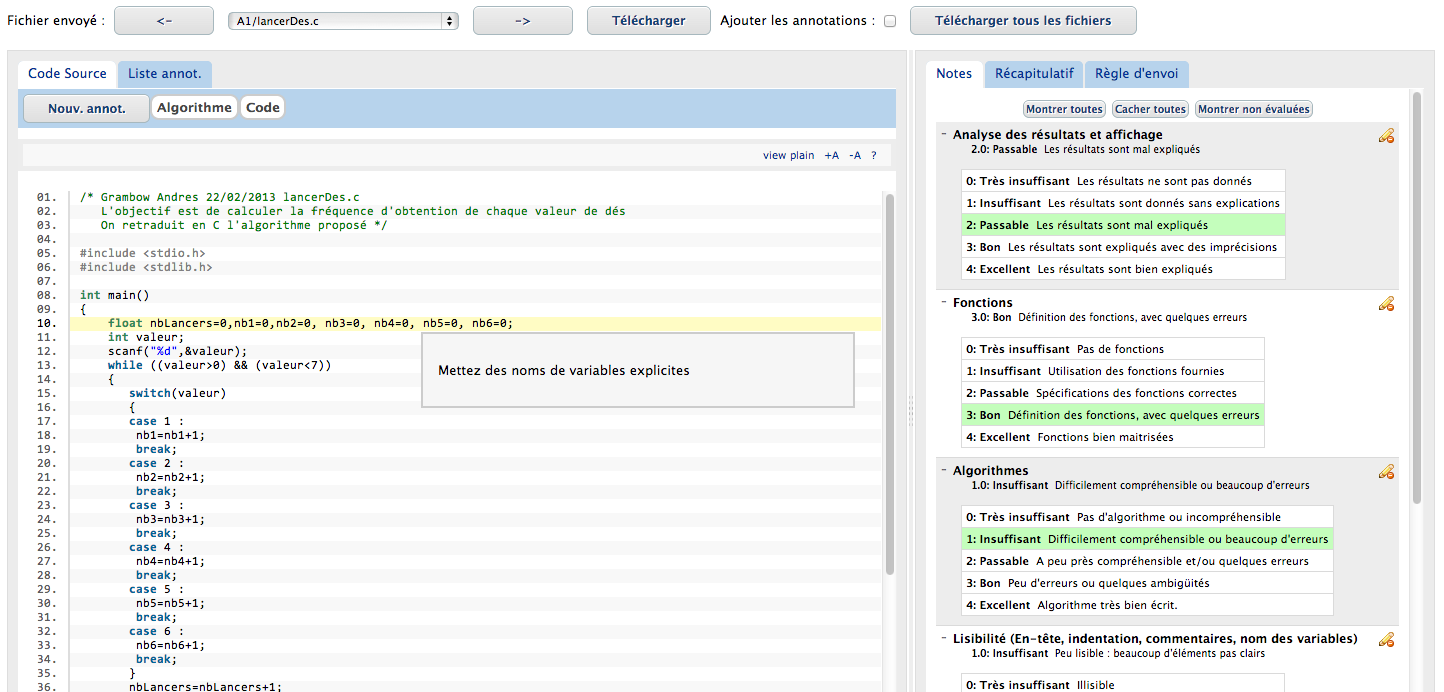
\includegraphics[width=\textwidth]{images/grader_view_fr.png}
                                }
                                %
                                \caption{Vue du correcteur}
                        \end{center}
                \end{figure}
        \end{block}
}

\frame{
        \frametitle{Quelques fonctionnalités}

        \begin{block}{Amélioration de l'enseignement (correcteur)}
                \begin{itemize}
                        \item Critères \textbf{fixes} d'évaluation
                        \item Annotations (code source, images et pdf)
                        \item Plusieurs correcteurs pour une copie
                        \item Gestion des correcteurs par critères
                \end{itemize}
                \vspace{-1em}
                \begin{figure}
                        \begin{center}
                                \scalebox{0.20}{
                                        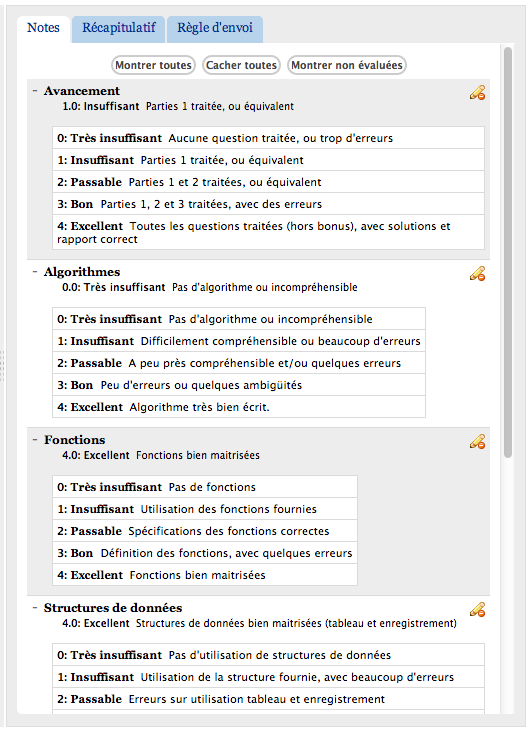
\includegraphics[width=\textwidth]{images/marks_fr.png}
                                }
                                %
                                \caption{Détermination de critères}
                        \end{center}
                \end{figure}
        \end{block}
}

\frame{
        \frametitle{Quelques fonctionnalités}

        \begin{block}{Amélioration de l'enseignement (correcteur)}
                \begin{itemize}
                        \item Prise en charge de plusieurs TP, dans l'idée d'une instance de MarkUs par matière
                        \item Gestion des \textbf{échéances} avec pénalités de retard (configurables)
                        \item Possibilité de voir et corriger une \textbf{ancienne} version
                \end{itemize}
        \end{block}
}

\frame{
        \frametitle{Quelques fonctionnalités}

        \begin{block}{Amélioration de l'enseignement (élève)}
                \begin{itemize}
                        \item Constitution des groupes \textbf{en fonction des TP}
                        \item Export des commentaires
                        \item Retour amélioré et plus rapide
                        \item Possibilité de revoir les commentaires
                		%%%%%%%
                		% TODO: faire un point sur les remark requets
                		%%%%%%%                        
                        \item Possibilité d'une \emph{remark request}
                \end{itemize}
                \vspace{-1em}
                \begin{figure}
                        \begin{center}
                                \scalebox{0.50}{
                                        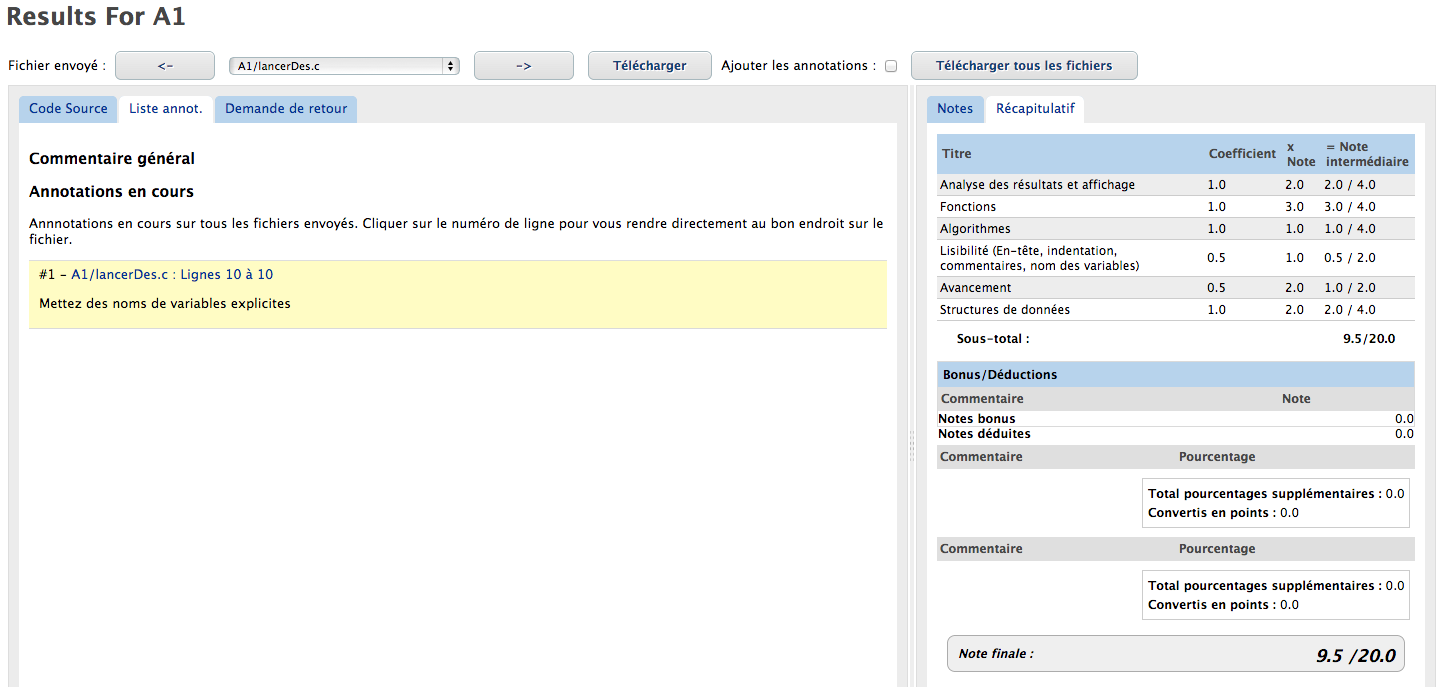
\includegraphics[width=\textwidth]{images/results_fr.png}
                                }
                                \caption{Vue des résultats par les étudiants}
                        \end{center}
                \end{figure}
        \end{block}
}

\frame{
        \frametitle{Quelques nouvelles fonctionnalités}

        \begin{exampleblock}{\emph{Release} de MarkUs 1.0}
                \begin{itemize}
                	\item Compatibilité avec Ruby 1.9.3 et Ruby on Rails 3.x
                	\item \textbf{Gestion des sections} au sein d'une promotion
                	\item Conversion des PDF \textbf{instantanée}
                	%%%%%%%
                	% TODO: faire un point sur les remark requets
                	%%%%%%%
                	\item Ajout des \emph{remark requests}
                	\item \textbf{Nouveau tableau de bord} pour l'administrateur
                \end{itemize}
%                \vspace{-1em}
%                \begin{figure}
%                        \begin{center}
%                                \scalebox{0.55}{
%                                        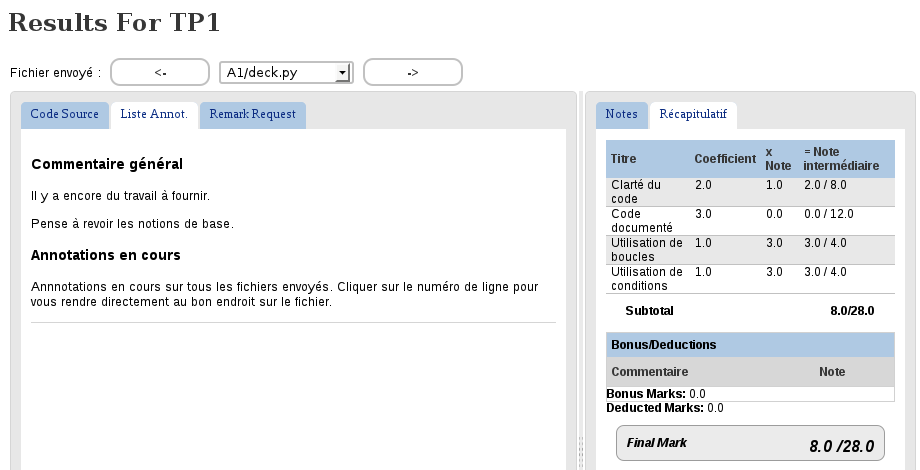
\includegraphics[width=\textwidth]{images/markus-commentaires.png}
%                                }
%                                \caption{Vue des résultats par les étudiants}
%                        \end{center}
%                \end{figure}
        \end{exampleblock}
}

\subsection*{Démonstration}

\frame{
        \frametitle{Démo}
        Et si nous passions à une petite illustration pratique\dots
}


\section{Impact sur l'enseignement et l'apprentissage}

% Cette partie pour donner un aperçu des fonctionnalités de MarkUs et leur impact sur l'enseignement

\subsection*{Avantages pour les enseignants}

\frame{
        \frametitle{Pourquoi MarkUs séduit les enseignants}
        \begin{itemize}
                \item Gestion de \textbf{gros volumes}
                \item Gestion \textbf{centralisée} des documents
                \item \textbf{Diminution du temps} de correction (environ 50\%)
                \item \textbf{Dématérialisation}
                \item Accès \textbf{nomade}
        \end{itemize}
}

\subsection*{Avantages pour les étudiants}

\frame{
        \frametitle{Pourquoi MarkUs séduit les étudiants}
        \begin{itemize}
                \item Une \textbf{unique} plate-forme de soumission et de correction
                \item Accès \textbf{permanent} aux anciens travaux annotés par les enseignants
                \item Amélioration du \textbf{délai} d'obtention de la correction
        \end{itemize}
}

\subsection*{Utilisation à Centrale Nantes}

\frame{
        \frametitle{Du côté de Centrale Nantes}
        
        \begin{block}{Déploiement du logiciel pour les cours d'informatique}
                \begin{itemize}
                        \item Depuis septembre 2010
                        \item Interconnecté avec \textbf{LDAP}
                        \item Utilisé en 1ère et 2e année :
                                \begin{itemize}
                                        \item 370 et 340 étudiants impactés
                                        \item 21 enseignants concernés
                                \end{itemize}
                        \item Enseignements d'\textbf{informatique} :
                                \begin{itemize}
                                        \item Algorithmique
                                        \item C
                                        \item Java
                                \end{itemize}
                \end{itemize}
        \end{block}
}

\frame{
        \frametitle{Les effets bénéfiques de MarkUs}
        \begin{block}{Côté étudiants :}
                \begin{itemize}
                        \item Effet pédagogique du \textbf{respect des dates limites}
                        \item Chaque \textbf{individu} accède à la correction du travail de son groupe
                        \item \textbf{Consultation accrue} des corrections laissées par les enseignants
                \end{itemize}
        \end{block}
}

\frame{
        \frametitle{Les effets bénéfiques de MarkUs}
        \begin{block}{Côté enseignants :}
                \begin{itemize}
                        \item Meilleure gestion \textbf{logistique}
                        \item Une première \textbf{uniformisation} des critères de correction
                        \item Aspect \textbf{incitatif} de la correction
                \end{itemize}
        \end{block}
}

\section{Déploiement de MarkUs}

\frame{
        \frametitle{Autour de MarkUs}
        \begin{block}{Modalités pratiques}
                \begin{itemize}
                        \item Écrit en Ruby, avec Ruby on Rails
                        \item Documents sauvegardés via Subversion
                        \item Accès via l'application web
                        \item Utilisateurs avancés : accès CLI via une API REST
                \end{itemize}
        \end{block}
        
        \begin{block}{Essayez le !}
                \begin{itemize}
                        \item Machine virtuelle : instance de MarkUs pré-configurée
                \end{itemize}
        \end{block}
}


\section{Conclusion}


\subsection*{Bilan}

\frame
{
        \frametitle{Synthèse}

        \begin{alertblock}{MarkUs, une application web d'annotation du code des étudiants}
                Comment améliorer la procédure d'évaluation des TP/projets d'étudiants ?
        \end{alertblock}

        \begin{block}{Usage de MarkUs}
                \begin{itemize}
                        \item Logiciel \textbf{libre}
                        \item Annotation du \textbf{code}, des \textbf{.pdf} et des \textbf{images}
                        \item Facilité de prise en main
                        \item Seul coût : installation et maintenance
                        \item Utilisation plébiscitée par les étudiants et les enseignants
%                        \item Vers la création de \textbf{cercles vertueux} : utilisateurs $\rightarrow$ contributeurs $\rightarrow$ mentors
                \end{itemize}
        \end{block}
}

\subsection*{Perspectives}

\frame{
        \frametitle{Améliorations à venir}

        \begin{block}{Vers un élargissement de l'utilisation de MarkUs}
                \begin{itemize}
%                        \item Analyse plus fine des effets du dispositif pédagogique
                        \item Module d'\textbf{annotation tactile}
                        \item Intégration d'annotations mathématiques
                        \item Tests automatiques du code envoyé par les étudiants
                        \item Élargissement à d'autres matières
                        \item Intégration à un \textbf{ENT} ?
                        \item Déploiement facilité à l'aide de machines virtuelles
                \end{itemize}
        \end{block}
}

\subsection*{Références}

\frame{
        \frametitle{Plus d'informations}

        \begin{block}{Liens et contacts}
                \begin{itemize}
                        \item Site du projet : \url{http://markusproject.org}
                        \item Essayer le logiciel en ligne : \url{http://demo.markusproject.org}
                        \item Sources : \url{https://github.com/MarkUsProject/Markus}
                        \item Blog EAT-TICE de l'Ecole Centrale de Nantes : \url{http://eat-tice.ec-nantes.fr}
                        \item Chan IRC : \#markus sur irc.freenode.net
                        \item Mailing list : \url{markus-dev@markusproject.org}
                \end{itemize}
        \end{block}
}

%\bibliography{biblio}
%\bibliographystyle{alpha}

\end{document}
